\documentclass[a4paper,12pt]{report}
\usepackage[utf8]{inputenc}
\usepackage[dutch]{babel}
\usepackage{geometry}
\usepackage{graphicx}
\usepackage{lmodern}
\usepackage{amsmath, amssymb}
\usepackage[T1]{fontenc}
\usepackage{xcolor}
\usepackage{color}
\usepackage{fancyvrb}
\usepackage{setspace}
\usepackage{tocbibind}
\usepackage{array} 
\usepackage{multicol}
\usepackage{tikz}
\usetikzlibrary{arrows.meta, positioning}
\usepackage[hidelinks]{hyperref}
\usepackage{titlesec} 
\usepackage{algorithm}
\usepackage{algpseudocode}


% \titleformat{\chapter}[display]
%   {\normalfont\huge\bfseries} % Format of chapter title
%   {\centering \fontsize{120pt}{140pt} \selectfont \thechapter} % Chapter number format
%   {0pt} % Space between chapter number and title
%   {\vspace{0.5em}\Huge \centering} % Line between number and title, and vertical space

% \titlespacing*{\chapter}{0pt}{-20pt}{20pt} % {left}{before}{after}




% \setlength{\cftbeforetoctitleskip}{-20pt} % Adjust space before ToC title
% % \setlength{\cftaftertoctitleskip}{20pt}  % Adjust space after ToC title


\setlength{\parskip}{0.8em}
\setlength{\parindent}{0pt}

\geometry{a4paper, top=2.5cm, bottom=2.5cm, left=2.5cm, right=2.5cm} 

\begin{document}

\begin{titlepage}
  \centering
  \vspace*{0cm}

  \Huge\textbf{Reinforcement Learning en Computerspellen} \\
  \vspace{1cm}
  \rule{\linewidth}{0.4mm}
  \Large
  Hoe beïnvloeden de specifieke kenmerken van computerspellen de effectiviteit van specifieke reinforcement learning-algoritmes?
  \rule{\linewidth}{0.4mm}

  \vspace{1.5cm}
  \includegraphics[width=0.2\textwidth]{logo-clz.png} \\
  \vspace{1.5cm}
  \large
  \textbf{Matthijs Gorter} \\
  \textbf{Thom Brinkhorst} \\
  \textbf{Pepijn van Iperen} \\
  \vspace{\fill}
  \normalsize

  Profielwerkstuk \\ onder begeleiding van \\ \textit{\textbf{S. Rook}} \\
  Christelijk Lyceum Zeist \\ Natuur en Techniek \\ Februari 2025 \\ \newpage
\end{titlepage}

\chapter*{Voorwoord}
\addcontentsline{toc}{chapter}{Voorwoord} % Voeg toe aan de inhoudsopgave
Voorwoord inhoud hier. Bedank mensen die geholpen hebben, beschrijf het doel van het profielwerkstuk en eventuele persoonlijke motieven of ervaringen.

\vspace{1cm}
\noindent
Matthijs Gorter, Thom Brinkhorst, Pepijn van Iperen \\
Christelijk Lyceum Zeist \\
Februari 2025

\chapter*{Variabelen en Notatie}
\addcontentsline{toc}{chapter}{Variabelen en Notatie} % Voeg toe aan de Inhoudsopgave
\begin{table}[h]
  \begin{tabular}{>{\raggedright}p{2.5cm} >{\raggedright\arraybackslash}p{10cm}}
    \textbf{Variabele}       & \textbf{Definitie}                                \\
    \rule{\linewidth}{0.4mm} & \rule{\linewidth}{0.4mm}                          \\
    $t$                      & Tijdstap                                          \\
    $T$                      & Laatste tijdstap van een episode (horizon)        \\
    $x$                      & Toestand (state)                                  \\
    $x_t$                    & Toestand op tijdstip $t$                          \\
    $x'$                     & Toestand een tijdstap na $x$                      \\
    $\mathcal{X}$            & Set van alle toestanden                           \\
    $a$                      & Actie                                             \\
    $\mathcal{A}$            & Alle mogelijke acties                             \\
    $a_t$                    & Actie op tijdstip $t$                             \\
    $r$                      & Beloning (reward)                                 \\
    $\mathcal{R}$            & Set van mogelijke beloningen                      \\
    $r_t$                    & Beloning op tijdstip $t$                          \\
    $r(x, a)$                & Beloningsfunctie                                  \\
    $\mu$                    & Deterministisch beleid                            \\
    $\pi$                    & Stochastisch beleid                               \\
    $\pi^*$                  & Optimale stochastisch beleid                      \\
    $\gamma$                 & Kortingsfactor tussen 0 en 1                      \\
    $p(x'|x, a)$             & Overgangswaarschijnlijkheidsfunctie               \\
    $\mathcal{P}$            & Overgangswaarschijnlijkheidsmatrix                \\
    $V(x)$                   & Waardefunctie                                     \\
    $Q(x, a)$                & Q-functie                                         \\
    $Q^*(x, a)$              & Q-functie met het optimale beleid                 \\
    $\mathbb{E}[X]$          & Verwachtingswaarde van variabele $X$              \\
    $\mathbb{E}[a|b]$        & Geconditioneerde verwachtingswaarde               \\
    $\mathbb{E}_{\pi}[X]$    & Verwachtingswaarde als beleid $\pi$ wordt gevolgd \\
  \end{tabular}
  \caption{Variabelen en Notatie}
\end{table}
\newpage

\tableofcontents

\chapter{Inleiding}
Introductie Onderwerp \\ Onderwerpkeuze verantwoorden \\
Onderzoeksvraag/Hoofdvraag met eventuele hypothese \\ Deelvragen \\ Wat zijn de
specifieke kenmerken van verschillende soorten computerspellen? \\ Welke
reinforcement learning-algoritmes zijn beschikbaar en wat zijn hun kenmerken?
\\ Hoe beïnvloeden de spelkenmerken de prestatie van reinforcement
learning-algoritmes? \\ klein stukje theorie als inleiding op het
theorie-onderdeel \\ werkplan in grote lijnen, opbouw van verslag \\

\chapter{Theoretisch Kader}

\section{Definitie}
Reinforcement Learning (RL) is een tak binnen kunstmatige intelligentie waarin
een agent leert door interactie met zijn omgeving. Een agent is een entiteit
die leert en acties onderneemt. Bij een zelfrijdende auto is het
besturingssysteem de agent, en bij een schaakspel is de schaker de agent. De
omgeving is alles waarmee de agent interageert en die reageert op de acties van
de agent. Bij een zelfrijdende auto is dit de weg waar de auto op rijdt en de
voertuigen om de auto heen. Bij een schaakspel is dit het schaakbord.

De agent leert door interactie met zijn omgeving. De agent ontvangt beloningen
of straffen (negatieve beloningen) als gevolg van zijn acties. Het doel van de
agent is om een strategie te ontwikkelen die de cumulatieve beloning
maximaliseert over tijd. Bij Super Mario Bros (1985) is Mario de agent en de
agent krijgt een beloning als Mario richting de eindslag beweegt (meestal naar
rechts) en als Mario een coin of een power up oppakt en Mario krijgt een straf
als Mario sterft en hij krijgt elke seconde straf zodat hij zo snel mogelijk
het level wilt voltooien.

Figuur~\ref{fig:rl_model} illustreert het basismodel van interactie binnen
Reinforcement Learning.
\begin{figure}[h]
  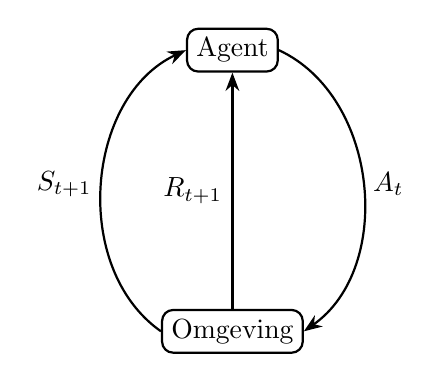
\begin{tikzpicture}[auto, thick, node distance=2cm,>=Stealth]
    \node[draw, rectangle, rounded corners] (agent) {Agent};
    \node[draw, rectangle, rounded corners, below=of agent, yshift=-1cm] (environment) {Omgeving};

    % Action arrow with adjusted bend
    \draw[->] (agent.east) to[bend left=60] node[midway, right] {$A_t$} (environment.east);

    % State arrow with adjusted text position
    \draw[->] (environment.north) to node[midway, left] {$R_{t+1}$} (agent.south);

    % Reward arrow with adjusted text position
    \draw[->] (environment.west) to[bend left=60] node[midway, left] {$S_{t+1}$} (agent.west);
  \end{tikzpicture}
  \caption{Reinforcement learning interactiemodel tussen agent en omgeving via acties, toestanden en beloningen.}
  \label{fig:rl_model}
\end{figure}

Een actie naar de beslissing die een agent neemt bij elke stap in een
besluitvormingsproces. Acties worden aangeduid met \( a \) en worden gekozen
uit een reeks mogelijke acties \( \mathcal{A} \). Elke door de agent genomen
actie beïnvloedt de interactie met de omgeving, wat leidt tot een verandering
in de toestand en een daaruit voortvloeiende beloning.

Een toestand \( x \) vertegenwoordigt de huidige situatie of staat van de
omgeving waarin de agent opereert. Dit wordt aangeduid met \( x \) en maakt
deel uit van de toestandsruimte \( \mathcal{X} \). Bij de aanvangsstap \( t = 0
\), begint de agent in een initiële toestand \( x_0 \) die willekeurig wordt
bepaald door een verdeling \( p \). Naarmate het proces vordert, bevindt de
agent zich in nieuwe toestanden gebaseerd op zijn acties.

Een beloning \( r \) is een feedbackwaarde die wordt ontvangen nadat de agent
een actie heeft uitgevoerd in een bepaalde toestand. Deze beloning wordt
bepaald door de beloningsfunctie \( r(x, a) \). De beloningsmatrix \( R \)
bevat de onmiddellijke beloningen voor elke combinatie van toestand en actie.

Een overgang beschrijft de verandering van de huidige toestand naar de volgende
toestand als gevolg van een actie die door de agent wordt genomen. De
waarschijnlijkheid van overgang wordt bepaald door de
overgangswaarschijnlijkheidsfunctie \( p(x'|x, a) \), die afhangt van de
huidige toestand \( x \), de genomen actie \( a \) en leidt tot een nieuwe
toestand \( x' \). De overgangswaarschijnlijkheidsmatrix \( P \) bevat de
waarschijnlijkheden van het overgaan van de ene toestand naar de volgende
toestand, gegeven een bepaalde actie.

\subsection{Markov-eigenschap}

MDP werkt onder de Markov-aanname, wat betekent dat de volgende toestand en beloning alleen afhangen van het huidige toestand-actiepaar en niet van enige eerdere geschiedenis. Deze eigenschap vereenvoudigt het besluitvormingsmodel door zich alleen te concentreren op de huidige situatie.

Voorbeeld van een MDP:
\begin{itemize}
    \item \textbf{Snake}: De toekomstige toestand (positie van de slang en voedsel) is volledig bepaald door de huidige toestand (huidige positie en locatie van het voedsel) en de actie (richting van beweging) zonder afhankelijk te zijn van de geschiedenis van eerdere bewegingen.
\end{itemize}

Voorbeeld van geen MDP:
\begin{itemize}
    \item \textbf{Poker}: De beslissingen in poker zijn afhankelijk van niet alleen de huidige hand, maar ook van de geschiedenis van inzetten en het gedrag van andere spelers in vorige rondes.
\end{itemize}

Voorbeeld van een twijfelgeval:
\begin{itemize}
    \item \textbf{Schaak}: Elke positie op het bord (toestand) en mogelijke zetten (acties) bepalen de volgende positie, maar strategieën kunnen afhankelijk zijn van eerdere zetten.
\end{itemize}

In een MDP gaat een agent verder in tijdstappen \(t = 0, 1, 2, \ldots, T\) waar de horizon \(T\) zowel eindig als oneindig kan zijn. Hierin is \(T\) oneindig tenzij anders aangegeven.

\subsection{Overgangswaarschijnlijkheidsmatrix}

Wanneer de set van alle toestanden \(\mathcal{X}\) en de set van alle acties \(\mathcal{A}\) eindig zijn, d.w.z. \(|\mathcal{X}|, |\mathcal{A}| < \infty\), kan de overgangswaarschijnlijkheidsfunctie \(p(x'|x,a)\) worden weergegeven als een overgangsmatrix.

De grootte van de overgangswaarschijnlijkheidsmatrix is \(|\mathcal{X}| \times |\mathcal{X}| \times |\mathcal{A}|\). Dit is een driedimensionale matrix. De dimensies zijn als volgt:
\begin{itemize}
    \item De huidige toestand \(x\).
    \item De genomen actie \(a\).
    \item De volgende toestand \(x'\).
\end{itemize}

\subsection{Beleid}

In RL is een beleid de strategie die een agent volgt om beslissingen te nemen. Het bepaalt welke actie een agent moet uitvoeren, gegeven de huidige toestand van de omgeving. Er zijn twee hoofdtypen beleid:

\begin{itemize}
    \item \textbf{Deterministisch Beleid}:
    \begin{itemize}
        \item \textbf{Formule:} \(a_t = \pi(s_t)\)
        \item \textbf{Beschrijving:} Voor elke toestand \(s_t\) kiest het beleid altijd dezelfde actie \(a_t\). Het resultaat is volledig voorspelbaar zolang de toestand bekend is.
    \end{itemize}
    
    \item \textbf{Stochastisch Beleid}:
    \begin{itemize}
        \item \textbf{Formule:} \(a_t \sim \pi(\cdot|s_t)\)
        \item \textbf{Beschrijving:} Voor een gegeven toestand \(s_t\) kiest het beleid een actie \(a_t\) volgens een waarschijnlijkheidsverdeling. Dit betekent dat de actie die wordt gekozen afhankelijk is van kans, wat leidt tot variabiliteit in het gedrag van de agent.
    \end{itemize}
\end{itemize}

\subsection{Verwachtingswaarde}

De verwachtingswaarde \(\mathbb{E}[X]\) (Expected value), of het gemiddelde, van een willekeurige variabele \(X\) is een manier om het gemiddelde resultaat te berekenen dat je zou verwachten als je een groot aantal experimenten uitvoert. Bijvoorbeeld, als \(X\) een dobbelsteenworp vertegenwoordigt, dan is \(\mathbb{E}[X]\) het gemiddelde van de uitkomsten 1, 2, 3, 4, 5, en 6, wat gelijk is aan 3,5.

\textbf{Geconditioneerde verwachtingswaarde} \(\mathbb{E}[a|b]\): het gemiddelde van \(a\) berekenen, gegeven de voorwaarde \(b\).

\subsection{Kortingsfactor}

De kortingsfactor \(\gamma\) is een getal tussen 0 en 1 dat het gewicht bepaalt van toekomstige beloningen ten opzichte van onmiddellijke beloningen. Bij een lage kortingsfactor hebben toekomstige beloningen weinig invloed. Bij een kortingsfactor van 1 hebben alle beloningen evenveel invloed.

\subsection{Waardefunctie}

De waardefunctie \(V(x)\) geeft de verwachte waarde van de totale beloning die een agent zal ontvangen vanaf de toestand \(x\) als hij het beleid \(\pi\) volgt.

\[
V(x) := \mathbb{E}_{\pi}\left[\sum_{t=0}^{\infty} \gamma^t r_t \mid x_0 = x\right]
\]

Hierin is \(\sum_{t=0}^{\infty} \gamma^t r_t\) de som van alle beloningen waarbij elke beloning wordt vermenigvuldigd met \(\gamma^t\) als de kortingsfactor (\(\gamma \in [0,1]\)). Dan wordt elke beloning met een groter tijdstapje (verder in de toekomst) kleiner en heeft dus minder invloed op de verwachte waarde.

\subsection{Q-functie}

De Q-functie \(Q(x,a)\) geeft de verwachte waarde van de totale beloning die een agent zal ontvangen vanaf de toestand \(x\) en na het nemen van actie \(a\), als hij daarna het beleid \(\pi\) volgt.

\[
Q(x,a) := \mathbb{E}_{\pi}\left[\sum_{t=0}^{\infty} \gamma^t r_t \mid x_0 = x, a_0 = a\right]
\]

\noindent waarin \(a_0 = a\) betekent dat de eerste actie \(a\) is.

De waardefunctie geeft aan hoe goed een bepaalde toestand is, terwijl de Q-functie aangeeft hoe goed een actie in een bepaalde toestand is.

Waarde functie en Q-functie zijn gerelateerd aan elkaar op deze manier:

\[
V(x) = \mathbb{E}_{a \sim \pi(\cdot|x)}[Q(x,a)]
\]

\subsection{Bellman vergelijking}

De Q-functie en de waardefunctie in RL moeten voldoen aan consistentievoorwaarden, bekend als de Bellman-vergelijkingen. Voor een gegeven beleid \(\pi\), kunnen de waardefunctie \(V(x)\) en de Q-functie \(Q(x,a)\) als volgt worden gedefinieerd:

\[
V(x) = \mathbb{E}_{a \sim \pi(\cdot|x), x' \sim p(\cdot|x,a)}[r(x,a) + \gamma V(x')]
\]

\[
Q(x,a) = \mathbb{E}_{x' \sim p(\cdot|x,a), a' \sim \pi(\cdot|x')}[r(x,a) + \gamma Q(x',a')]
\]

\noindent waarin:
\begin{itemize}
    \item \(a \sim \pi(\cdot|x)\) betekent dat actie \(a\) de actie is volgens beleid \(\pi\) in toestand \(x\).
    \item \(x' \sim p(\cdot|x,a)\) betekent dat toestand \(x'\) volgt uit toestand \(x\) en actie \(a\) volgens de overgangswaarschijnlijkheidsfunctie \(p\).
    \item \(a' \sim \pi(\cdot|x')\) betekent dat de volgende actie \(a'\) de actie is volgens beleid \(\pi\) in de nieuwe toestand \(x'\).
    \item \(r(x,a)\) is de beloning van actie \(a\) in toestand \(x\).
\end{itemize}

\subsection{Evaluatie en Controle}

Er zijn twee problemen in RL:
\begin{itemize}
    \item \textbf{Evaluatie:} Het eerste probleem in RL is evaluatie. Het doel is om te berekenen hoe goed een bepaald beleid \(\pi\) presteert. Dit wordt gedaan door te kijken naar de waarde functie \(V(x)\) of de Q-functie \(Q(x,a)\).
    
    Waarom is evaluatie een probleem?
    \begin{itemize}
        \item \textbf{Complexiteit van de omgeving:} In een dynamische omgeving kan het moeilijk zijn om te voorspellen welke beloningen een agent zal ontvangen vanuit een bepaalde toestand, vooral als de omgeving verandert zonder dat de agent verandert.
        \item \textbf{Variabiliteit van beloningen:} Beloningen kunnen stochastisch zijn, wat betekent dat dezelfde actie in dezelfde toestand verschillende uitkomsten kan hebben.
        \item \textbf{Lange termijn effecten:} Het effect van een bepaalde actie wordt pas later zichtbaar.
    \end{itemize}
    
    Het evaluatieprobleem wordt meestal beschouwd als een subroutine van het tweede probleem: controle.
    
    \item \textbf{Controle:} Bij controle is het doel om het beleid \(\pi\) te vinden dat de waarde functie maximaliseert over de initiële toestanden \(x \sim \rho\).
    
    \[
    \max_{\pi} \mathbb{E}_{x \sim \rho}[V(x)]
    \]
    
    \noindent waarin \(x \sim \rho\) betekent dat de toestand \(x\) van de agent komt uit een vooraf gedefinieerde verzameling toestanden, waarbij elke toestand een bepaalde kans heeft om gekozen te worden.
    
    Waarom is controle een probleem?
    \begin{itemize}
        \item \textbf{Exploratie vs. exploitatie:} De agent moet een balans vinden tussen het verkennen van nieuwe acties om betere beloningen te ontdekken (exploratie) en het uitbuiten van bekende acties die momenteel de hoogste beloning bieden (exploitatie).
        \item \textbf{Dimensionale complexiteit:} In veel RL-toepassingen zijn er een groot aantal toestanden en acties, wat het zoeken naar het optimale beleid computationeel duur maakt.
    \end{itemize}
    
    Het optimale beleid \(\pi^*\) is het beleid dat de verwachte cumulatieve beloning over tijd maximaliseert.
    
    \[
    Q^*(x,a) = \mathbb{E}_{x' \sim p(\cdot|x,a)}\left[r(x,a) + \gamma \max_{a'} Q^*(x',a')\right]
    \]
\end{itemize}

\section{Belangrijke Algoritmes}



\section{Artificiële Leermethodes}

\section{Computerspellen}

\chapter{Onderzoeksmethoden}

\chapter{Analyse en Resultaten}

\chapter{Conclusie}

\chapter{Discussie}

\chapter{Referentielijst}

\chapter{Bijlagen}

\end{document}
